\def\null{\texttt{NULL}}
\def\makeset{$\mathop{\mathit{makeset}}(x)$}
\def\find{$\mathop{\mathit{find}}(x)$}
\def\union{$\mathop{\mathit{union}}(x, y)$}

\section{Union-find}

\paragraph{Popis.}

% Sú problémy, ktoré vyžadujú spájanie objektov do množín a množín navzájom 
% a následné určovanie, do ktorej množiny objekt patrí. Od takejto \emph{
% dátovej štruktúry pre disjunktné množiny} očakávame, že si bude udržiavať 
% jednoznačného \emph{zástupcu} každej množiny a bude poskytovať 
% tieto tri oprácie: 
V niektorých aplikáciach potrebujeme udržiavať prvky rozdelené do skupín
(disjunktných množín), pričom skupiny sa môžu zlučovať a my potrebujeme
pre daný prvok efektívne zistiť, do ktorej skupiny patrí. Predpokladáme,
že každá množina $S$ je jednoznačne určená jedným svojim zástupcom $x\in S$
a potrebujeme implementovať nasledovné tri operácie:

\begin{itemize}
\item \makeset\ -- vytvorí novú množinu $S=\{x\}$ s jedným prvkom; %,
                   %ktorý nepatrí do žiadnej inej množiny;
\item \union\ -- ak $x,y$ sú zástupcovia množín $S$ a $T$,
                 {\it union} vytvorí novú množinu $S\cup T$,
                 pričom $S$ aj $T$ zmaže. Zástupcom novej množiny $S\cup T$
                 je $x$ alebo $y$.
\item \find\ -- nájde zástupcu množiny, v ktorej sa 
                prvok $x$ nachádza.
\end{itemize}

V takejto situácií je vhodná štruktúra \emph{union-find}.
% Vďaka častej asociácií objektov a spájania množín ako vrcholy a hrany grafu 
% sa často dátová štruktúra abstraktne reprezentuje ako 
% \emph{les} -- množina zakorenených stromov. 
% Konkrétnou implementáciou potom býva pole objektov -- vrcholov. Ku každému 
% objektu sa musí udržiavať smerník $p(x)$ na otca v strome. Smerník zástupcu 
% množiny ukazuje na hodnotu \null.
Táto dátová štruktúra sa reprezentuje ako les, kde každý strom zodpovedá
jednej množine a korene stromov sú zástupcovia množín. Pri implementácií si
stačí pre každý prvok $x$ udržiavať smerník $p(x)$ na jeho otca
(pre koreň je $p(x)=\null$).

Operácia \makeset\ teda vytvorí nový prvok $x$ a nastaví $p(x) = \null$. 

Operáciu \find\ vykonáme tak, že budeme sledovať cestu po smerníkoch, až 
kým nenájdeme zástupcu. 

Operáciu \union\ ide najjednoduchšie vykonať tak, že presmerujeme smerník 
$p(y)$ na prvok $x$, teda $p(y) = x$. 
Môžeme ľahko pozorovať, že takýto \emph{naivný} spôsob je neefektívny, 
lebo nám operácia \find\ v najhoršom prípade, na $n$ prvkoch, trvá $O(n)$ 
krokov. 

\paragraph{Použitie.}

Union-find sa dá použiť na reprezentáciu neorientovaného grafu,
do ktorého pridávame hrany a odpovedáme na otázku "sú dané dva
vrcholy spojené nejakou cestou?" (t.j.\ sú v rovnakom komponente súvislosti?).
Medzi najznámejšie aplikácie patria Kruskalov algoritmus na nájdenie najlacnejšej
kostry \citep{kruskal} a unifikácia \citep{unif}.

\citet{cholesky} ukázali, ako sa dá union-find použiť pri Choleského dekompozícií
riedkych matíc. Autori navrhli efektívny algoritmus, ktorý zistí počet nenulových
prvkov v každom riadku a stĺpci výslednej matice, čo slúži na efektívnu alokáciu
pamäte.

Pre offline verziu úlohy, kde sú všetky operácie dopredu známe, \citep{offline-uf}
navrhli lineárny algoritmus. Článok obsahuje tiež viacero aplikácií v teoretickej
informatike.

\smallskip
Existujú dva prístupy ako zlepšiť operácie a tým aj zrýchliť ich vykonanie. 
Sú to: heuristika \emph{spájanie podľa ranku} a rôzne heuristiky na 
\emph{kompresiu cesty}. 

%\begin{figure}
%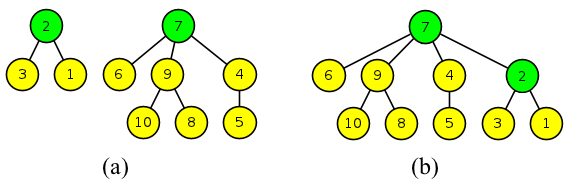
\includegraphics[width=\columnwidth]{obrazky/union.png}
%\caption{\emph{Spájanie podľa ranku.} (a) Pred spojením. (b) Po spojení. 
%Plytší strom sa napojil pod hlbší.} 
%\label{img:union} 
%\end{figure}
\paragraph{Heuristika na spájanie.}

Prvá heuristika pridáva ku algoritmom hodnotu 
$rank(x)$, ktorá bude určovať najväčšiu možnú hĺbku podstromu zakorenenú 
vrcholom $x$. V tom prípade pri o\-pe\-rá\-cií \makeset\ zadefinujeme 
$rank(x) = 0$. 
Pri o\-pe\-rá\-cií \union\ vždy porovnáme $rank(x)$ a $rank(y)$, aby sme zistili, 
ktorý zástupca predstavuje menší strom. Smerník tohto zástupcu potom napojíme 
na zástupcu s výšším rankom. Zástupca novej množiny bude ten s vyšším rankom. 
Ak sú oba ranky rovnaké, vyberieme ľubovoľného zo zástupcov $x$ a $y$, 
jeho rank zvýšime o jeden a smerník ostatného zástupcu bude ukazovať 
na tohto zástupcu. Zástupcom novej množiny bude vybratý zástupca. 

\paragraph{Heuristiky na kompresiu cesty.}

\begin{figure}
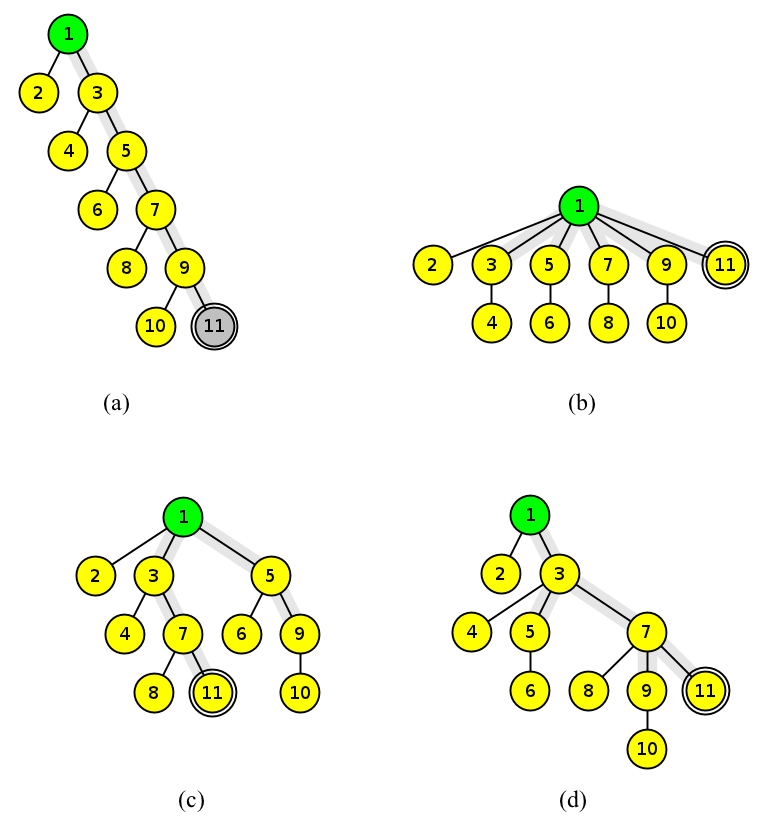
\includegraphics[width=\columnwidth]{obrazky/komp.png}
\caption{\emph{Kompresia cesty z vrcholu 11 do koreňa.} 
Cesta je vyznačená šedou. 
(a) Pred vykonaním kompresie. Pri úplnej kompresii~(b) sa všetky vrcholy 
napoja na zástupcu. Pri delení cesty~(c) a pólení cesty~(d) sa cesta skráti 
približne na polovicu.} 
\label{img:komp} 
\end{figure}

Druhou heuristikou je kompresia cesty. Algoritmov na efektívnu kompresiu 
cesty je veľa \citep{paths2}, tu popíšeme tie najefektívnejšie. Prvou z nich 
je \emph{úplná kompresia} \citep{comp1}. Pri vykonávaní operácie \find, po tom, 
ako nájdeme zástupcu, napojíme všetky vrcholy po ceste priamo pod koreň. Toto 
síce trochu spomalí prvé hľadanie, ale výrazne zrýchli ďalšie hľadania pre
všetky prvky na ceste ku koreňu.
Druhou heuristikou je \emph{delenie cesty} \citep{comp2}. Pri vykonávaní 
operácie \find\ pripojíme každý vrchol v ceste od vrcholu $x$ po koreň stromu
na otca jeho otca. Treťou heuristikou je \emph{pólenie cesty} \citep{comp2}.
Pri vykonávaní operácie \find\  pripojíme každý druhý vrchol v ceste od vrcholu
$x$ po koreň stromu na otca jeho otca. Kompresie sú znázornené v obrázku~%
\ref{img:komp}.

Časová zložitosť union-findu záleží od toho, koľko prvkov je v množinách a koľko je 
operácií celkovo vykonaných operácií. Všetky uvedené spôsoby ako vykonať 
operáciu \find\ sa dajú použiť s obomi realizáciami operácie \union. 
Počet prvkov označme $n$ a počet operácií $m$. V praxi je zvyčajne počet 
operácií oveľa väčší ako počet prvkov. Pri tomto predpoklade ($m\geq n$) je 
pri použití spájania podľa ranku časová zložitosť pre algoritmus bez kompresie 
$\Theta(m\log n)$ a pre všetky tri uvedené typy kompresií 
$\Theta(m\mathop{\alpha}(m,n))$ \citep{paths2}.

\paragraph{Vizualizácia.} Union-find sme vizualizovali ako les. Pre názorné 
oddelenie množín sme si zvolili pravidlo, ktoré zakazovalo vykresliť vrchol 
napravo od najľavejšieho vrcholu a naľavo od napravejšieho vrcholu inej 
množiny. Jednotlivé množiny sme už vykreslovali tesným Walkerovým algoritmom 
\citep{walker}. Vizualizácie poskytuje všetky vyššie spomínané heuristiky a 
aj tlačidlo na vykonanie viacerých náhodných spojení naraz. Toto je užitočné, 
keď chce uživateľ vidieť, ako dátová štruktúra vyzerá, po vykonaní 
veľa operácií.

% V tabuľke~\ref{fig:uf:comp} je porovnanie časových zložitostí \citep{paths2}.

% \begin{table}
% \centering
% \small
% %\footnotesize %toto tu mám nechať?
% \subfloat[Časová zložitosť pre union-find, keď $m \geq n$.][Prehľad časových zložitostí, ak $m \geq n$.]{
% \begin{tabular}{m{2.5cm}m{2.2cm}m{2.2cm}}
% & Naivné spájanie & Spájanie podľa ranku \tabularnewline
% \hline
% Naivné hľadanie & $\Theta\left( mn\right)$ & $\Theta\left( m\log n\right)$ \tabularnewline
% Úplná kompresia, delenie cesty, pólenie cesty & $\Theta\left(m\log _{1+m/n} n \right)$ & $\Theta\left( m\alpha\left( m, n\right) \right)$ \tabularnewline
% \label{fig:uf:comp1}
% \end{tabular}
% }
% \qquad
% \subfloat[Časová zložitosť pre union-find, keď $m < n$.][Prehľad časových zložitostí, ak $m < n$.]{
% \begin{tabular}{m{2.5cm}m{2.2cm}m{2.2cm}}
% & Naivné spájanie & Spájanie podľa ranku \tabularnewline
% \hline
% Naivné hľadanie & $\Theta\left( mn\right)$ & $\Theta\left(n + m\log n\right)$ \tabularnewline
% Úplná kompresia& $\Theta\left(n + m\log  n \right)$ & $\Theta\left(n + m\alpha\left( n, n\right) \right)$ \tabularnewline
% Delenie cesty & $\Theta\left(n \log m \right)$ & $\Theta\left(n + m\alpha\left( n, n\right) \right)$ \tabularnewline
% Pólenie cesty & $\Omega\left(n + m\log n \right)$, $O\left(n\log m\right)$ & $\Theta\left(n + m\alpha\left( n, n\right) \right)$ \tabularnewline
% \label{fig:uf:comp2}
% \end{tabular}}
% \caption{\normalsize Porovnanie časových zložitostí pre rôzne kombinácie hľadaní prvkov a 
% spájaní množín pre union-find. Počet prvkov je $n$ a počet operácií je $m$. $\alpha$ 
% je inverzná Ackermannova funkcia. V praxi zväčša platí, že $m > n$.}
% \label{fig:uf:comp}
% \end{table}

%citovat Walkerov alg. - to mám robiť tu?

